\documentclass[11pt]{article}
\usepackage[margin=1in]{geometry}
\usepackage{booktabs}
\usepackage{graphicx}
\usepackage{xcolor}
\usepackage{tikz}
\usetikzlibrary{positioning,fit,backgrounds}
\usepackage{enumitem}
\usepackage{fancyhdr}
\usepackage{titlesec}
\usepackage{lmodern}
\usepackage[colorlinks=true,linkcolor=black,urlcolor=blue!50!black,citecolor=black]{hyperref}
\hypersetup{pdftitle={Hyperfinance Agent},pdfauthor={Team hyper.}}

\definecolor{ink}{RGB}{30,32,36}
\definecolor{accent}{RGB}{38,98,217}
\definecolor{soft}{RGB}{245,246,248}
\definecolor{line}{RGB}{210,214,220}

\titleformat{\section}{\large\bfseries\color{ink}}{\thesection}{0.8em}{}
\titleformat{\subsection}{\normalsize\bfseries\color{ink}}{\thesubsection}{0.8em}{}
\setlist{nosep,leftmargin=1.4em}
\pagestyle{fancy}
\fancyhf{}
\renewcommand{\headrulewidth}{0pt}
\fancyfoot[C]{\small\color{ink!60}Hyperfinance Agent --- agentic accounting system \quad\textbar\quad \thepage}

\title{\vspace{-1.5em}\textbf{Hyperfinance Agent}\\[0.2em]\large An Agentic Accounting System with Deterministic Financial Engines\\ and Bounded Human Authority}
\author{Team hyper.\thanks{Built at HackMIT 2026. Repository: \texttt{github.com/MatthewKim323/hyper.}}}
\date{September 19, 2026}

\begin{document}
\maketitle
\vspace{-1em}

\begin{abstract}
\noindent General-purpose LLM agents can read financial evidence, but left alone they produce narrative conclusions that cannot be audited, replayed, or safely authorized. Hyperfinance Agent separates \emph{investigation} from \emph{calculation} and \emph{authorization}: agents retrieve evidence and propose work, deterministic engines recompute every amount and enforce blocking conditions, and only verified humans can attest evidence or approve outcomes. Around this core we built a voice-first workspace where a persistent agent workforce investigates anomalies over a company's real data surface, raises structured concerns to humans, converts completed work into governed reusable skills, and renders live financial artifacts. We report honest worker-baseline measurements on four public accounting benchmarks---Invoice Sandbox (18/18 customer totals, \$0.00 aggregate error), DABstep (7/10), BenchRec (95.8\% precision, 91.2\% recall), and APEX (70/89 rubric criteria under a GPT-6 Astra judge)---and we are explicit that these measure the isolated agent harness, not yet the full backend-controlled system.
\end{abstract}

\section{Why this exists}

Accounting work done by an unconstrained LLM fails in a specific way: it writes prose. ``The invoice looks fine'' is not a payable proposal; ``these match'' is not a reconciliation. Amounts must be reconstructed from records, discrepancies must be proven against rules, and anything that moves money requires a human decision bound to the exact artifact being approved.

The design premise of Hyperfinance Agent is therefore \textbf{not} ``a smarter agent.'' It is a division of labor:

\begin{itemize}
\item \textbf{Agents are good at} searching messy evidence, noticing anomalies, drafting hypotheses, and doing new kinds of work.
\item \textbf{Code is good at} integer arithmetic, three-way matching, cumulative credit checks, residual computation, and refusing ambiguous input.
\item \textbf{Humans are good at} attesting that a record is real, and deciding whether a proposed journal or payable amount may proceed.
\end{itemize}

Every surface in the system is built to keep those roles from blurring. Agents cannot approve. Engines cannot guess. Humans approve hash-bound artifacts, not vibes.

\section{System architecture}

\begin{figure}[h]
\centering
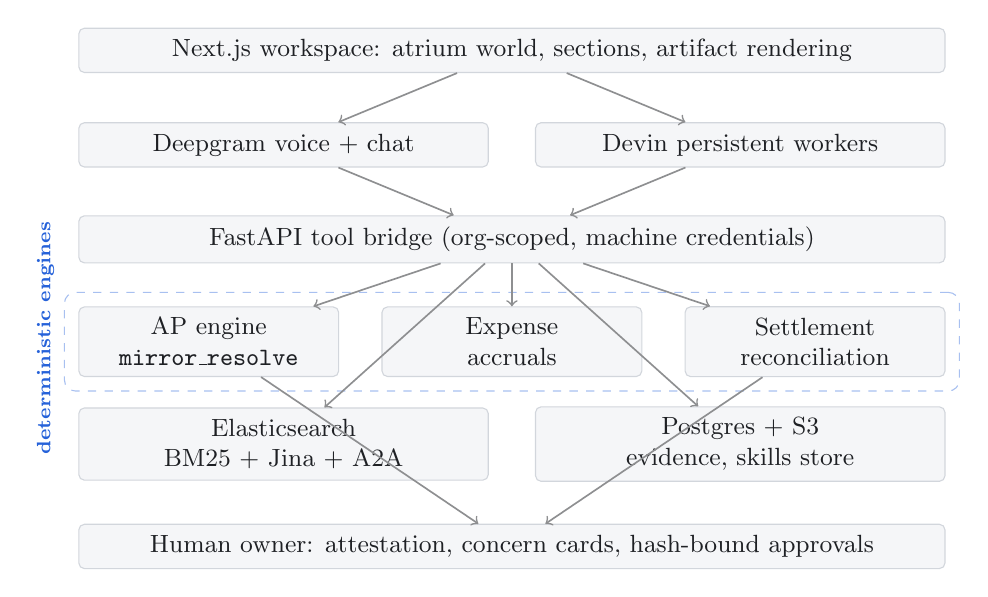
\begin{tikzpicture}[
  box/.style={draw=line,fill=soft,rounded corners=2pt,minimum height=1.5em,inner sep=4pt,font=\small,text=ink,align=center},
  lbl/.style={font=\scriptsize\bfseries\color{accent}},
  arr/.style={->,draw=ink!50,semithick}
]
\node[box,minimum width=11cm] (ui) at (0,0) {Next.js workspace: atrium world, sections, artifact rendering};
\node[box,minimum width=5.2cm] (voice) at (-2.9,-1.2) {Deepgram voice + chat};
\node[box,minimum width=5.2cm] (devin) at (2.9,-1.2) {Devin persistent workers};
\node[box,minimum width=11cm] (bridge) at (0,-2.4) {FastAPI tool bridge (org-scoped, machine credentials)};
\node[box,minimum width=3.3cm] (ap) at (-3.85,-3.7) {AP engine\\ \texttt{mirror\_resolve}};
\node[box,minimum width=3.3cm] (acc) at (0,-3.7) {Expense\\ accruals};
\node[box,minimum width=3.3cm] (set) at (3.85,-3.7) {Settlement\\ reconciliation};
\node[box,minimum width=5.2cm] (es) at (-2.9,-5.0) {Elasticsearch\\ BM25 + Jina + A2A};
\node[box,minimum width=5.2cm] (pg) at (2.9,-5.0) {Postgres + S3\\ evidence, skills store};
\node[box,minimum width=11cm] (human) at (0,-6.3) {Human owner: attestation, concern cards, hash-bound approvals};

\begin{scope}[on background layer]
\node[draw=accent!40,dashed,rounded corners=4pt,fit=(ap)(acc)(set),inner sep=5pt] (engs) {};
\node[lbl,rotate=90,anchor=south] at (engs.west) {\;deterministic engines};
\end{scope}

\draw[arr] (ui) -- (voice);
\draw[arr] (ui) -- (devin);
\draw[arr] (voice) -- (bridge);
\draw[arr] (devin) -- (bridge);
\draw[arr] (bridge) -- (ap);
\draw[arr] (bridge) -- (acc);
\draw[arr] (bridge) -- (set);
\draw[arr] (bridge) -- (es);
\draw[arr] (bridge) -- (pg);
\draw[arr] (ap) -- (human);
\draw[arr] (set) -- (human);
\end{tikzpicture}
\caption{Layered architecture. Agents investigate through a bounded tool bridge; engines compute; humans authorize.}
\end{figure}

\subsection{Interfaces and orchestration}

The user-facing surface is a Next.js workspace (the ``atrium'') with a voice agent (Deepgram listen--think--speak with a configurable managed think model; the code defaults to GPT-4o mini) and dashboard sections for cases, evidence, activity, review, and benchmarks. Behind it, a FastAPI backend runs a durable dispatcher that manages persistent Devin workers---at most two concurrent cloud sessions per organization, under cumulative session and ACU budgets.

Agents never hold user credentials. Each worker session receives a scoped machine token (\texttt{APP\_AGENT\_TOKEN}, only its hash stored) and reaches the backend exclusively through an authenticated tool bridge: \texttt{GET /agents/tool-definitions} and \texttt{POST /agents/tools}. Workers cannot delegate, cannot modify cases, cannot respond as the user, and cannot touch other organizations. Every delegation, event, and case update is recorded transactionally with request-key idempotency.

\subsection{Evidence and retrieval}

Connectors (Gmail, Drive, Ramp, Plaid) ingest read-only source material into Postgres/S3, indexed into Elasticsearch with hybrid retrieval (BM25 + semantic embeddings via Jina, reciprocal-rank fusion, optional Jina reranking). Beyond search, the backend delegates \emph{investigations} to Elastic Agent Builder over the A2A protocol: the Elastic agent iteratively discovers related records through bounded ES|QL tools whose organization constraint is fixed in the tool definition, not supplied by the model. Returned findings are validated by our backend---chunk ownership, current source status, citation integrity---before becoming concerns.

\subsection{Deterministic engines}

The product's core is three engines that accept only strict, normalized evidence and return exact results or explicit blockers:

\textbf{Accounts payable} (\texttt{mirror\_resolve} + \texttt{/accounting} API). Three-way matching across invoice, purchase order, receipt, agreement, and credit records, all in integer minor units (USD/EUR/GBP, no FX). Analysis requires invoice-minus-verified-credits to agree with received-quantity-at-supported-price; a price credit cannot settle a quantity exception. Proposals are hash-bound drafts validated by code (\texttt{engine:deterministic\_validator}); approval is a separate owner action bound to the exact result hash, and replacing a backing source invalidates dependent proposals.

\textbf{Expense accruals} (\texttt{/accounting/accruals}). From three immutable packets---contract/rate/account mapping, deliveries, and the complete posted ledger---the engine filters at month-end cutoff, computes quantity $\times$ rate, subtracts net posted expense including validated reversals, and emits a balanced journal proposal plus next-day reversal. It stays unposted until owner approval; subsequent posting, reversal, and invoice observations are tracked as lifecycle evidence.

\textbf{Settlement reconciliation} (\texttt{/accounting/settlements}). Proves a processor batch's arithmetic (sales, refunds, fees, reserves $\rightarrow$ payout) and its bank-statement match independently, with identity, duplicate, coverage, and completeness checks. Content-hashed runs are durable; verified bank transactions cannot be reused across runs.

Across all three: unsupported fields are rejected rather than discarded, uncertain evidence blocks rather than guesses, and no engine route can post to an external ledger or move money.

\subsection{Human authority}

Three distinct checkpoints keep authority with people:

\begin{itemize}
\item \textbf{Attestation.} Only an organization owner can mark a structured source row as verified evidence (\texttt{OWNER\_VERIFIED}, verifier \texttt{human:<clerk-subject>}). An LLM cannot promote its own extraction to trusted input.
\item \textbf{Concern cards.} When agents hit ambiguity or missing evidence they raise concerns; Jev generates a card with three checked options plus a custom response. Cards never approve journals---they resolve questions.
\item \textbf{Hash-bound approval.} Every approvable artifact (payable proposal, accrual, reconciliation) is approved against its exact result hash. There is no agent tool for approval at all.
\end{itemize}

\subsection{Learned skills}

Completed workflows become procedural memory. The lifecycle: discover existing skill $\rightarrow$ research gaps $\rightarrow$ implement and execute in the worker's isolated workspace $\rightarrow$ save execution logs $\rightarrow$ save an immutable draft package (SKILL.md generated by the service; scripts/tests/references as integrity-checked resources) $\rightarrow$ record a run report $\rightarrow$ owner reviews the actual tests and evidence and activates $\rightarrow$ retrieval on similar tasks. Failure reports quarantine active versions immediately. Skills are org-scoped packages in Postgres metadata + S3 storage, indexed summary-only in Elasticsearch with a SQL fallback. The backend never executes skill code; self-reported passes are labeled as such, and activation is the independent promotion gate.

\subsection{Artifacts}

For live financial visuals, agents call a composition tool backed by json-render: Jev emits a fixed three-node spec (chart type, points typed actual/projected, decimal strings) which the frontend renders with bklit charts---fast enough for in-conversation projections.

\section{Evaluation}

\subsection{Method}

We measured \textbf{isolated worker baselines} on four public accounting benchmarks: each run uploads inputs only to a fresh Devin cloud session with no Hyperfinance Agent backend tools, no answer keys, and an ACU cap; grading keys and scorers stay local; prompts and input archives are hash-pinned. We report every run, including a mid-run ACU suspension.

\subsection{Results}

\begin{table}[h]
\centering\small
\begin{tabular}{@{}llll@{}}
\toprule
\textbf{Benchmark} & \textbf{Workload} & \textbf{Result} & \textbf{Grading} \\
\midrule
Invoice Sandbox & 112 PDFs, 18 customers & \textbf{18/18 totals, \$0.00 error} & pinned native scorer \\
DABstep (dev) & 10 questions, 138k rows & \textbf{7/10} (6/7 hard passed) & pinned native scorer \\
BenchRec v3 & 32,048 bank rows & \textbf{95.8\% precision / 91.2\% recall} & custom metrics \\
APEX (dev) & 10 month-end tasks & \textbf{70/89 criteria, 0.710 macro} & GPT-6 Astra judge \\
\bottomrule
\end{tabular}
\end{table}

\noindent BenchRec matchers execute in a locked-down container (no network, read-only, pinned image) before scoring. DABstep passed 1/3 easy and 6/7 hard tasks in the original run. The original APEX worker hit its 10-ACU cap before emitting output and required a follow-up message. Its initial GPT-4.1 grade (71/89) contained an internally inconsistent numerical-tolerance verdict. A fresh \texttt{gpt-6-astra} assessment of the unchanged answers yields 70/89 criteria and 71.0\% macro task score. The old grades are preserved; changing the judge is not an agent improvement. This remains a provisional local model judgment, not expert or official grading.

\subsection{Same-data baselines and repeated trials}

The BenchRec version-3 distribution includes \texttt{MatcherByChatGPT\_submission.csv}. We scored it locally with the same exact-allocation metric and all 32,048 expected bank IDs. Its zero-or-one-element prediction arrays were normalized without selecting among guesses. The filename does not establish the underlying model, prompt or compute budget. It is a distributed reference submission, not a verified frontier-model baseline.

\begin{center}
\small
\begin{tabular}{@{}lrrr@{}}
\toprule
\textbf{BenchRec method} & \textbf{Precision} & \textbf{Recall} & \textbf{Coverage} \\
\midrule
Distributed reference & 95.20\% & 62.20\% & 64.90\% \\
Original Devin worker & 95.83\% & 91.22\% & 94.56\% \\
Verified-v2, mean of 3 trials & 96.23\% & 88.72\% & 91.58\% \\
Unique exact-total rules & 99.51\% & 46.48\% & 46.40\% \\
Exact-reference conservation rules & 99.86\% & 8.70\% & 8.66\% \\
\bottomrule
\end{tabular}
\end{center}

Verified-v2 adds source-grounded checklists, executable calculations and cross-checks, allocation conservation, interpretation of the supplied manuals, and final-output review. Three fresh trials per benchmark were authorized under 60 ACU of total configured caps. Inputs are unchanged; no prior answers or grading feedback are supplied. BenchRec gains 0.40 precision percentage points on average but loses 2.50 recall points; none of its three trials reaches 99.8\% precision. DABstep scores 7/10, 6/10 and 7/10 (66.67\% mean), versus the original 70\%: no improvement is demonstrated. All three APEX candidate sessions stopped at their 10-ACU caps without complete outputs: completion is 0/3 and all three attempts remain ungraded. They were not resumed or granted higher caps; this differs from the original baseline's completion nudge and prevents a clean candidate accuracy comparison.

A separate post-hoc conservation gate on the original BenchRec assignments raises precision only to 95.92\% while reducing recall to 84.92\%. This negative result shows that balanced amounts are insufficient to establish identity. The rules-only precision result likewise cannot be presented without its low recall. Source-only DABstep diagnostics identified count-versus-volume denominators, null wildcard handling, and unsupported fine thresholds as concrete targets for executable checks rather than further prompt expansion.

\subsection{Published comparisons and limitations}

The \href{https://huggingface.co/blog/dabstep}{DABstep launch report} gives historical hard-test baselines, including approximately 16\% for o3-mini. These are neither current frontier results nor comparable to our ten-question development split. The \href{https://www.mercor.com/apex/apex-accounting-leaderboard/}{APEX leaderboard} evaluates 160 private tasks across ten worlds; its current headline table reports 61.0\% for Fable 5.1 and 60.0\% for GPT-6 Astra. Different inputs, task isolation, harnesses and graders prohibit claiming that our public-development scores beat those systems.

Repeated public-fixture trials measure variation, not held-out generalization. The original baseline has one run; provider-managed worker models are not pinned. Repeated questions are correlated, not additional independent tasks. Missing outputs stay in the attempted denominator. No run uses Hyperfinance Agent's accounting APIs or learned skills; the next product-level comparison must exercise that real tool bridge. Cloud answer-key isolation is instruction-based, not a firewall. New judge caches bind model, protocol, rubric and answer hashes and never overwrite legacy grades. Current checks passed 22 focused runner/scorer tests and all 323 evaluation tests.

\section{Current state and limitations}

Implemented and test-covered: the full tool bridge and dispatcher, all three engines with owner-only approval paths, the learned-skill lifecycle with quarantine, Elastic A2A delegation with backend citation validation, concern cards, artifacts, and the benchmark harness itself.

Not yet proven live: Clerk-authenticated onboarding end-to-end, the Elastic A2A path against a provisioned agent (credentials pending), a live Devin session through a public tunnel, and Postgres-backed aggregates outside the compose stack. BenchRec precision (95.8\%) shows real headroom on high-precision matching. The engines deliberately cover narrow ground: whole-unit records, USD/EUR/GBP, no taxes, no FX, no split deposits, no external posting.

\section{Conclusion}

Hyperfinance Agent treats accounting agents as investigators operating under engineering controls, not as oracles. The measurable claim today is a competent isolated worker; the architectural claim---which the benchmark harness is built to test next---is that binding agent proposals to deterministic engines and hash-bound human approval converts fluent output into auditable financial work.

\end{document}
